\documentclass[11pt]{article}

\usepackage{url}
\usepackage{hyperref}
\usepackage{graphicx}
\usepackage{verbatim}
\usepackage{color}
\setlength{\parskip}{0.5cm plus4mm minus3mm}
\usepackage{upquote}
\usepackage{float}
\usepackage{subcaption}

\textwidth=6.4in
\textheight=8.5in
\hoffset=-0.7in
\voffset=-0.7in

\setlength{\parindent}{0cm} 

\newcommand{\Yfun}{Y}
%\newcommand{\TAG}{test}
\newcommand{\TAG}{\begin{color}{blue}This tutorial is currently under construction. Please check back later for more by keeping your software updated.\end{color}}

\newcommand{\HERE}{\begin{color}{blue}Currently working on this part.\end{color}}

\hyphenation{Text-Wrangler}

\title{Chapter 4: Vector Spherical Harmonics}
\author{Kylee Ford, Sarah Kroeker, Alain Plattner}

\begin{document}
\maketitle

\section{Representation 2 of Vector Fields}

The second representation of vector fields include $E_{lm}$, $F_{lm}$, and $C_{lm}$.

$E_{lm}$: vector components from the gradient of a potential field from a planet. \\
$F_{lm}$: vector components from the gradient of a potential field from outside the satellite radius (space). \\
$C_{lm}$: same as in representation 1.

\subsection{Building Vector Spherical Harmonics:} 
Let's calculate the spherical harmonic functions first for $E_{lm}$.  We will need to set some parameters:

\verb|L = 2;|\\
\verb|theta = 0:0.01:pi;|\\
\verb|phi = 0:0.01:2*pi;|

We can now calculate the spherical harmonic functions by running:

\verb|[E,theta,phi] = elm(L,theta,phi+pi);|

This provides \verb|E|, which contains the three components of the $E_{lm}$ vector spherical harmonics for degrees $l=0$ to $l=L$.   \verb|E{1}| contains $(L+1)^2$ pixel maps for the radial component.  Each row of \verb|E{1}| is a pixel map represented as a vector of numbers.  \verb|E{2}| contains $(L+1)^2$ pixel maps for the colatitudinal components and \verb|E{3}| contains $(L+1)^2$ pixel maps for the longitudinal components.  From the \verb|help| function, we can see that \verb|elm| function provides the pixel map values in the \textit{addmout} format.  

Let's plot the radial component of $E_{lm}$ with \verb|l=2| and \verb|m=-1|.  With the \textit{addmout} format, this is the sixth row, which is denoted as \verb|E{1}(6,:)|.  Our first step would be to label the radial, colatitudinal, and longitudinal components.  The best way to do this would be to also create an index such that we can change it easily:

\verb|index = 6;|\\
\verb|E2m1_rad = E{1}(index,:);|\\
\verb|E2m1_theta = E{2}(index,:);|\\
\verb|E2m1_phi = E{3}(index,:);|

Now we can reshape this into a pixel matrix of size length(theta) by length(phi) by running: 

\verb|E2m1_rad_matrix = reshape(E2m1_rad,length(theta),length(phi));|

Now we can plot \verb|E2m1_rad| on the Mallweide projection:

\verb|plotplm(E2m1_rad_matrix,phi,pi/2-theta,1)|\\
\verb|kelicol(1)|

We can also plot the colatitudinal component with the same (l,m).  We will need to reshape this as above and plot:

\verb|E2m1_theta_matrix = reshape(E2m1_theta,length(theta),length(phi));|\\
\verb|plotplm(E2m1_theta_matrix,phi,pi/2-theta,1)|

Plot the longitudinal component by running:

\verb|E2m1_phi_matrix = reshape(E2m1_phi,length(theta),length(phi));|\\
\verb|plotplm(E2m1_phi_matrix,phi,pi/2-theta,1)|

Compare your plots to figure 1.

\begin{figure}[H]
  \begin{subfigure}{.5\textwidth}
  \centering
  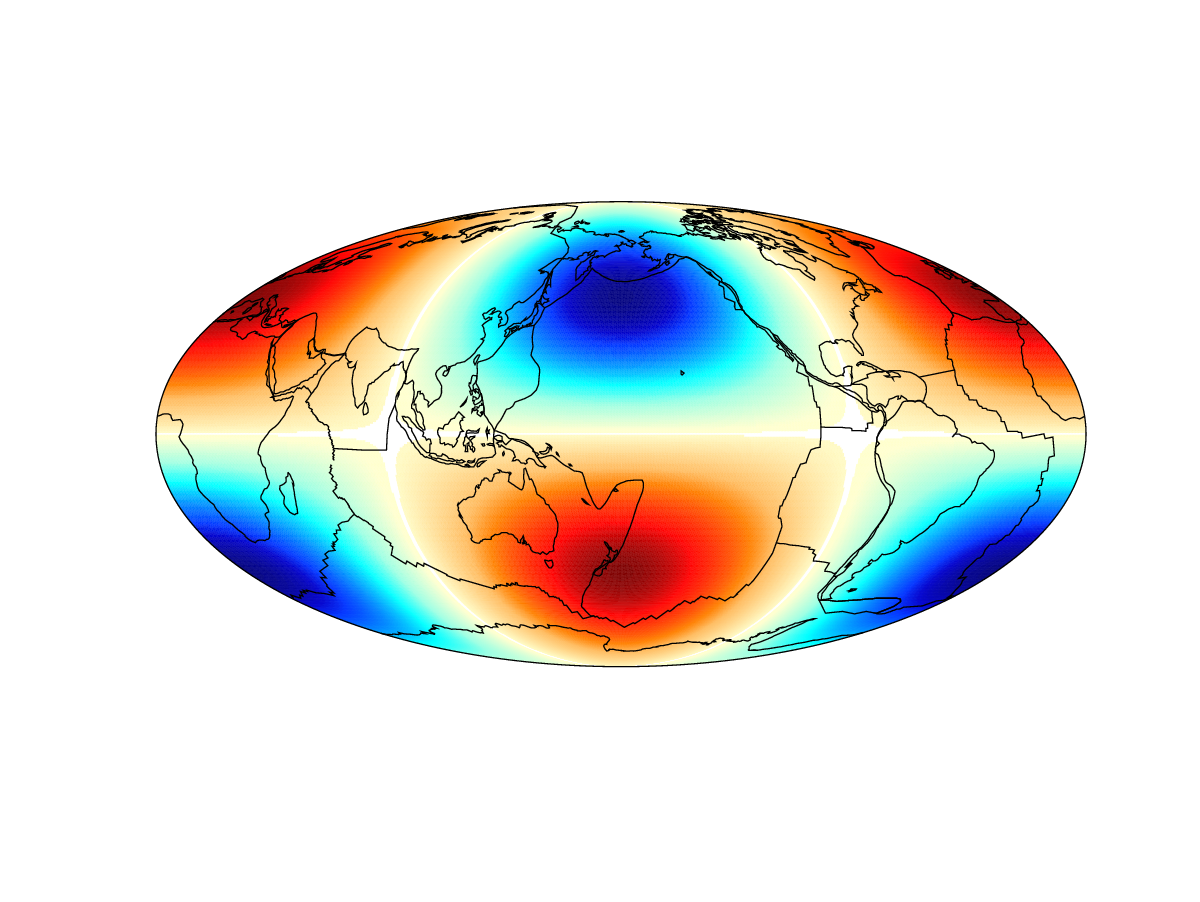
\includegraphics[width=0.8\textwidth]{figures_Rep2/E2m1_rad.png}
  \caption{Radial component}
  \label{rad}
  \end{subfigure}
  \begin{subfigure}{.5\textwidth}
  \centering
  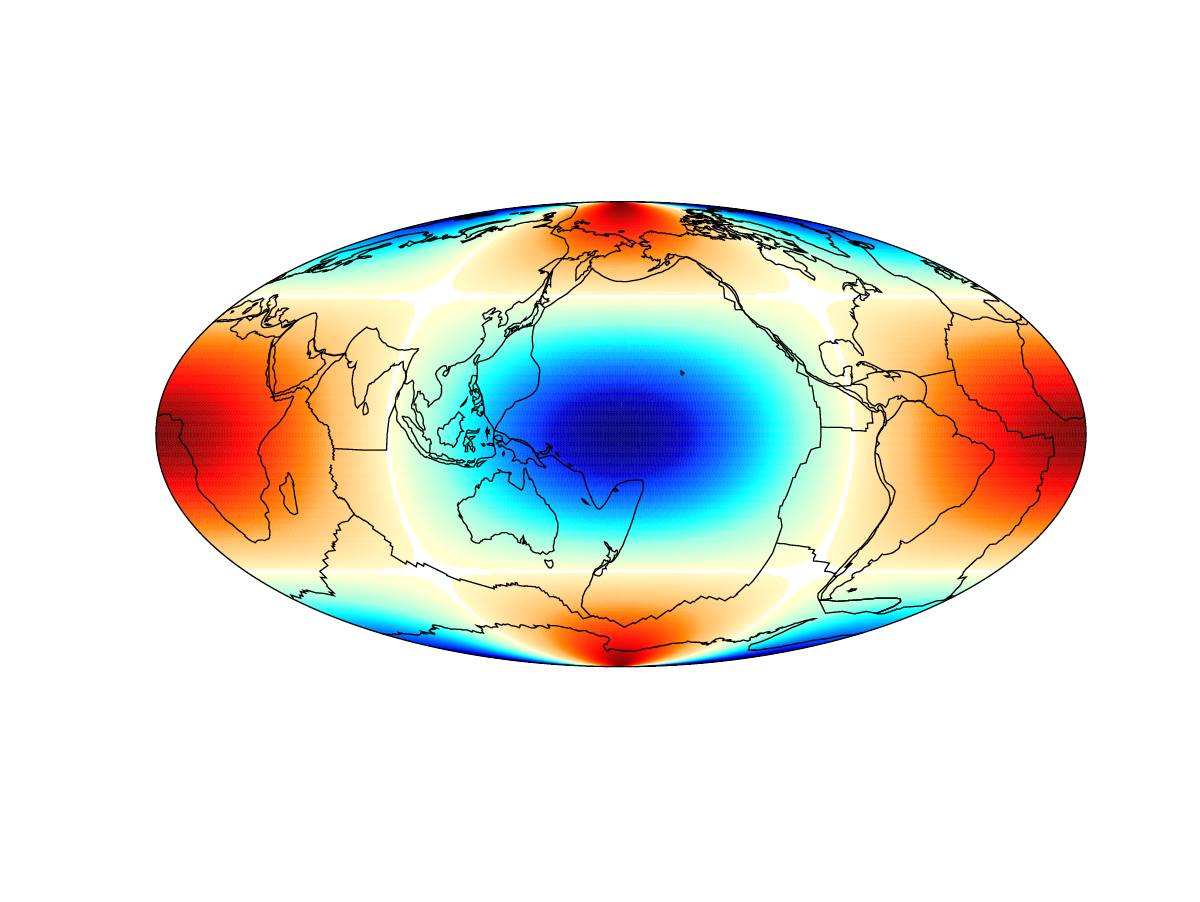
\includegraphics[width=0.8\textwidth]{figures_Rep2/E2m1_theta.png}
  \caption{Colatitudinal component}
  \end{subfigure}
  \begin{subfigure}{.5\textwidth}
  \centering
  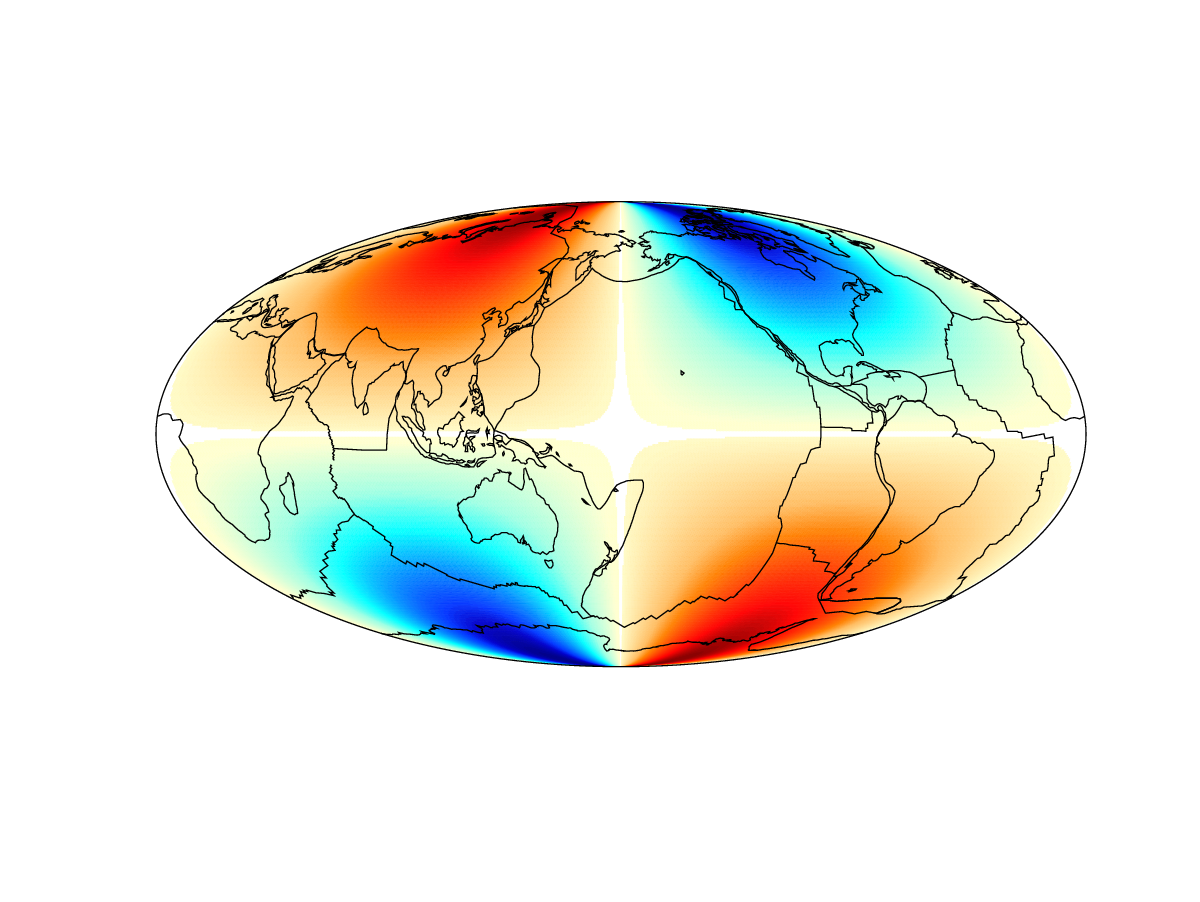
\includegraphics[width=0.8\textwidth]{figures_Rep2/E2m1_phi.png}  
  \caption{Longitudinal component}
  \end{subfigure}
  \caption{Vector spherical harmonic with $E_{2-1}$ plot of the radial component in (a), colatitudinal component in (b), and the longitudinal component in (c).}
\label{E6}
\end{figure}

We can also plot each component on one figure.  To do this, we will need to use a function called \verb|quiver|, which can be used as the \verb|help| function describes.  We will need a lower resolution to start with, so change theta and phi to:

\verb|theta = 0:0.1:pi;|\\
\verb|phi = 0:0.1:2*pi;|

You will need to recalculate $E_{lm}$ as well.  After this, open a new figure and run the following:

\verb|plotplm(E2m1_rad_matrix,phi,pi/2-theta,4)|\\
\verb|kelicol(1)|\\
\verb|caxis([-1,1]*max(abs(caxis)))|\\
\verb|hold on|\\
\verb|quiver(phi*180/pi,90-theta*180/pi,E2m1_phi_matrix,E2m1_theta_matrix,'k','LineWidth',1)|\\
\verb|hold off|

Compare your result to figure 2.

\begin{figure}[H]
  \centering
  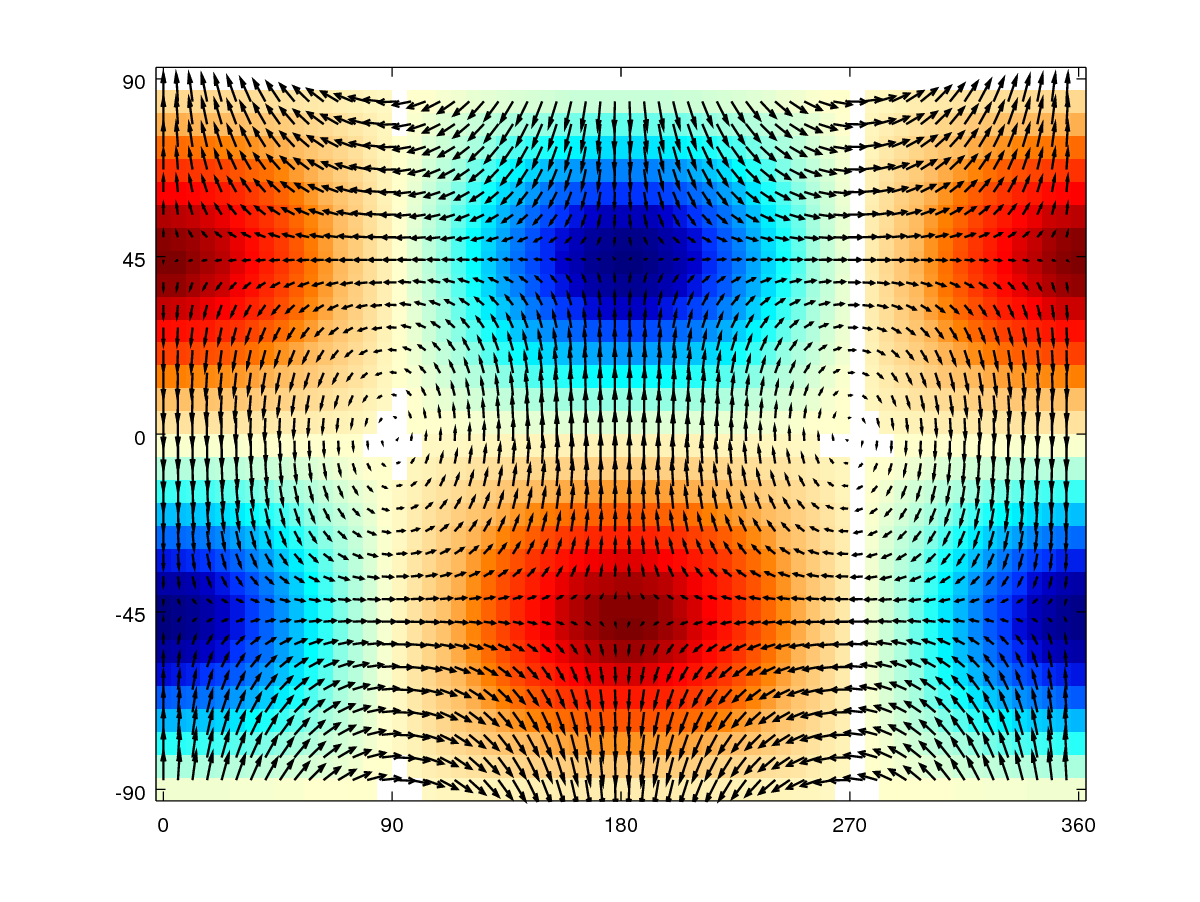
\includegraphics[width=0.8\textwidth]{figures_Rep2/E2m1_quiver.png}  
  \caption{Vector spherical harmonic with $E_{2-1}$.}
\label{E6_quiver}
\end{figure}

\textbf{Exercise:} We can plot another (l,m), say $E_{20}$, which would be the the seventh row in $E_{lm}$.  

\verb|index = 7;|\\
\verb|E20_rad = reshape(E{1}(index,:),length(theta),length(phi));|\\
\verb|E20_theta = reshape(E{2}(index,:),length(theta),length(phi));|\\
\verb|E20_phi = reshape(E{3}(index,:),length(theta),length(phi));|

Let's plot with the \verb|quiver| function again:

\verb|plotplm(E20_rad,phi,pi/2-theta,4)|\\
\verb|kelicol(1)|\\
\verb|caxis([-1,1]*max(abs(caxis)))|\\
\verb|hold on|\\
\verb|quiver(phi*180/pi,90-theta*180/pi,E20_phi,E20_theta,'k','LineWidth',1)|\\
\verb|hold off|

Compare your plot to figure 3.

\begin{figure}[H]
  \centering
  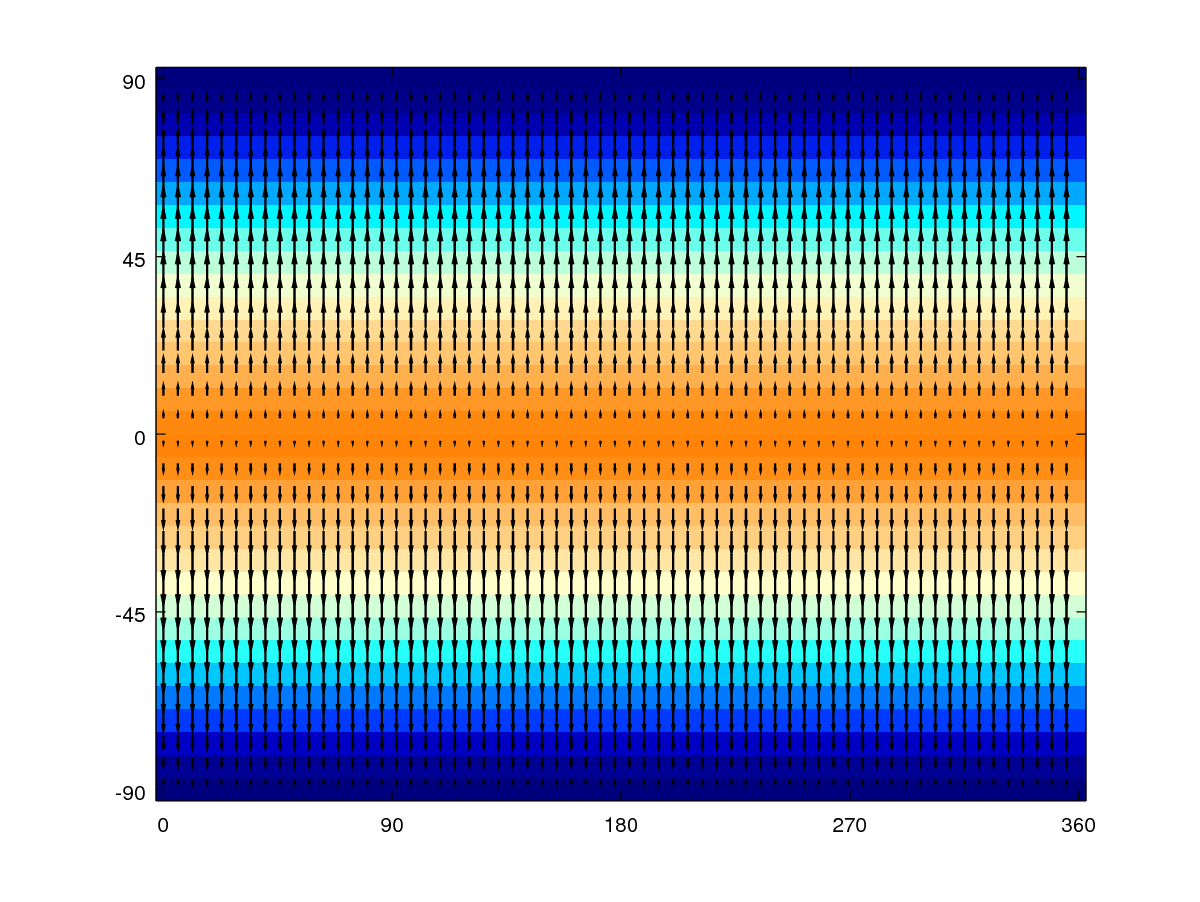
\includegraphics[width=0.5\textwidth]{figures_Rep2/E20_quiver.png}  
  \caption{Vector spherical harmonic $E_{20}$.}
\label{E7}
\end{figure}

\textbf{Exercise:} Try some of your own $E_{lm}$ functions with different l and m values.

\subsection{Linear Combinations of Vector Spherical Harmonics}

Let's try a linear combination of vector spherical harmonics, choose: $2E_{00}-1.5E_{10}+3E_{11}$.  We can plot this in a couple different ways, either by first reshaping each of the $E_{lm}$ values then make the linear combination or make the linear combination first then reshape it.  Try both and compare the results.  For the sake of computation, let's try the second way.  We will need to choose our parameters then calculate the linear combination:

\verb|L = 2;|\\
\verb|theta = 0:0.1:pi;|\\
\verb|phi = 0:0.1:2*pi;|\\
\verb|[E,theta,phi] = elm(L,theta,phi+pi);|\\
\verb|lincomb_rad = 2*E{1}(1,:)-1.5*E{1}(3,:)+3*E{1}(4,:);|\\
\verb|linr_rad = reshape(lincomb_rad,length(theta),length(phi));|\\
\verb|lincomb_theta = 2*E{2}(1,:)-1.5*E{2}(3,:)+3*E{2}(4,:);|\\
\verb|linr_theta = reshape(lincomb_theta,length(theta),length(phi));|\\
\verb|lincomb_phi = 2*E{3}(1,:)-1.5*E{3}(3,:)+3*E{3}(4,:);|\\
\verb|linr_phi = reshape(lincomb_phi,length(theta),length(phi));|\\

Now we can plot:

\verb|plotplm(linr_rad,phi,pi/2-theta,4);|\\
\verb|kelicol(1)|\\
\verb|caxis([-1,1]*max(abs(caxis)))|\\
\verb|hold on|\\
\verb|quiver(phi*180/pi-180,90-theta*180/pi,linr_phi,linr_theta,'k','LineWidth',1)|\\
\verb|hold off|

Compare your plot to figure 4.

\begin{figure}[H]
  \centering
  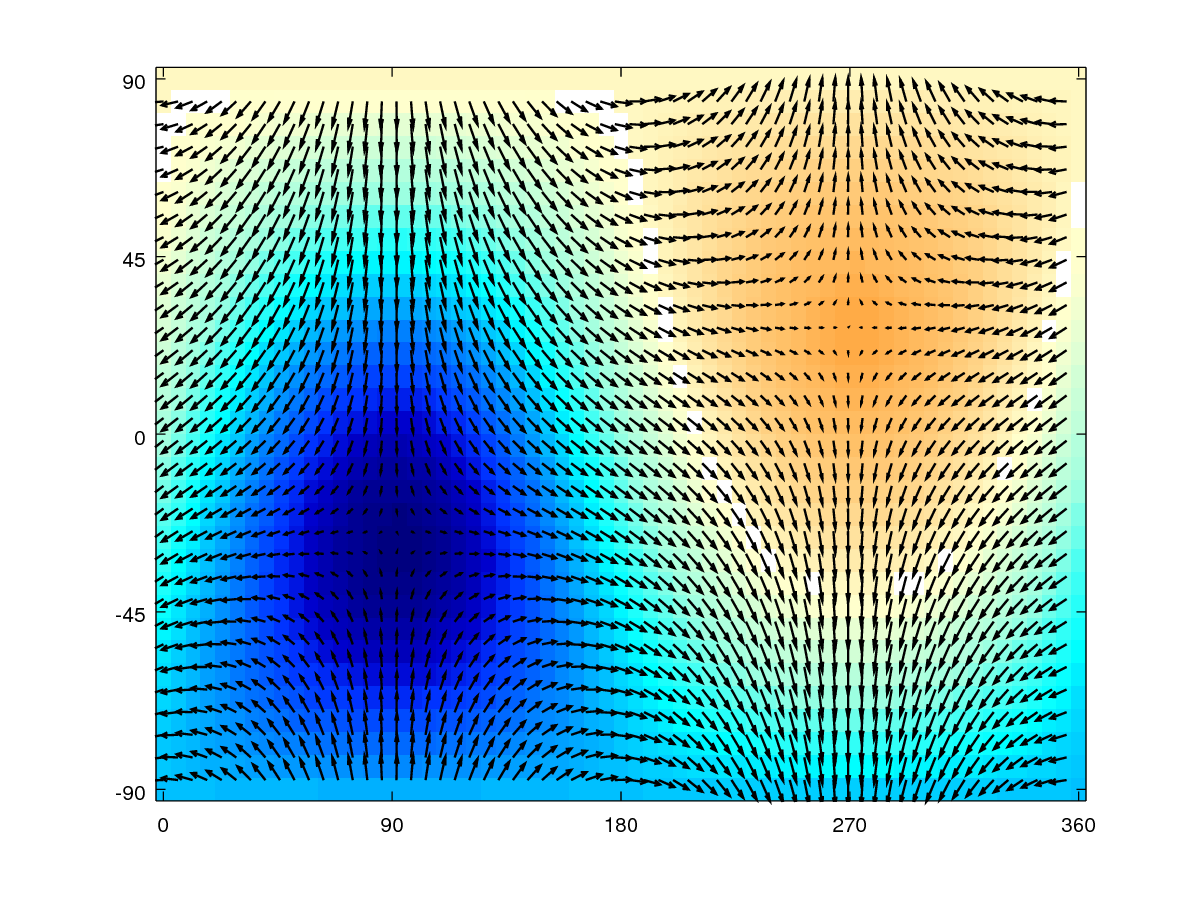
\includegraphics[width=0.5\textwidth]{figures_Rep2/lincomb1.png}  
  \caption{Linear combination of the vector spherical harmonics $2E_{00}-1.5E_{10}+3E_{11}$.}
\label{E_comb}
\end{figure}

\subsubsection{Building Spherical Harmonics with known Coefficients:}

If we know the spherical harmonic coefficients (aka the coefficients in the linear combination as above), we can build spherical harmonics in a different way. We first will need to put the coefficients in the following format:

\verb|Elmcosi = [l,m,cosine expansion coefficient,sine expansion coefficient]|

The cosine and sine expansion coefficients are determined by whether m is positive, negative, or zero.  As described in Plattner and Simons (2017) in equation (2), we know that if m is negative or zero, the coefficient is the cosine portion and if m is positive, the coefficient is the sine portion.  So for our linear combination $2E_{00}-1.5E_{10}+3E_{11}$, we can create the matrix:

\verb|Elmcosi = [0,0,2,0 ; 1,0,-1.5,0 ; 1,1,0,3]|

From these coefficients, we can build the spherical harmonic functions through the \verb|elm2xyz| function.  This will give us a cell array with the radial, colatitudinal, and longitudinal components.  Run:

\verb|[Elm,phi,theta] = elm2xyz(Elmcosi,5);|

Now we can plot these, as we did above:

\verb|plotplm(Elm{1},phi,pi/2-theta,4);|\\
\verb|kelicol(1)|\\
\verb|caxis([-1,1]*max(abs(caxis)))|\\
\verb|hold on|\\
\verb|quiver(phi,theta,Elm{3},Elm{2},'k','LineWidth',1)|\\
\verb|hold off|

Compare your plot to figure 5.

\begin{figure}[H]
  \centering
  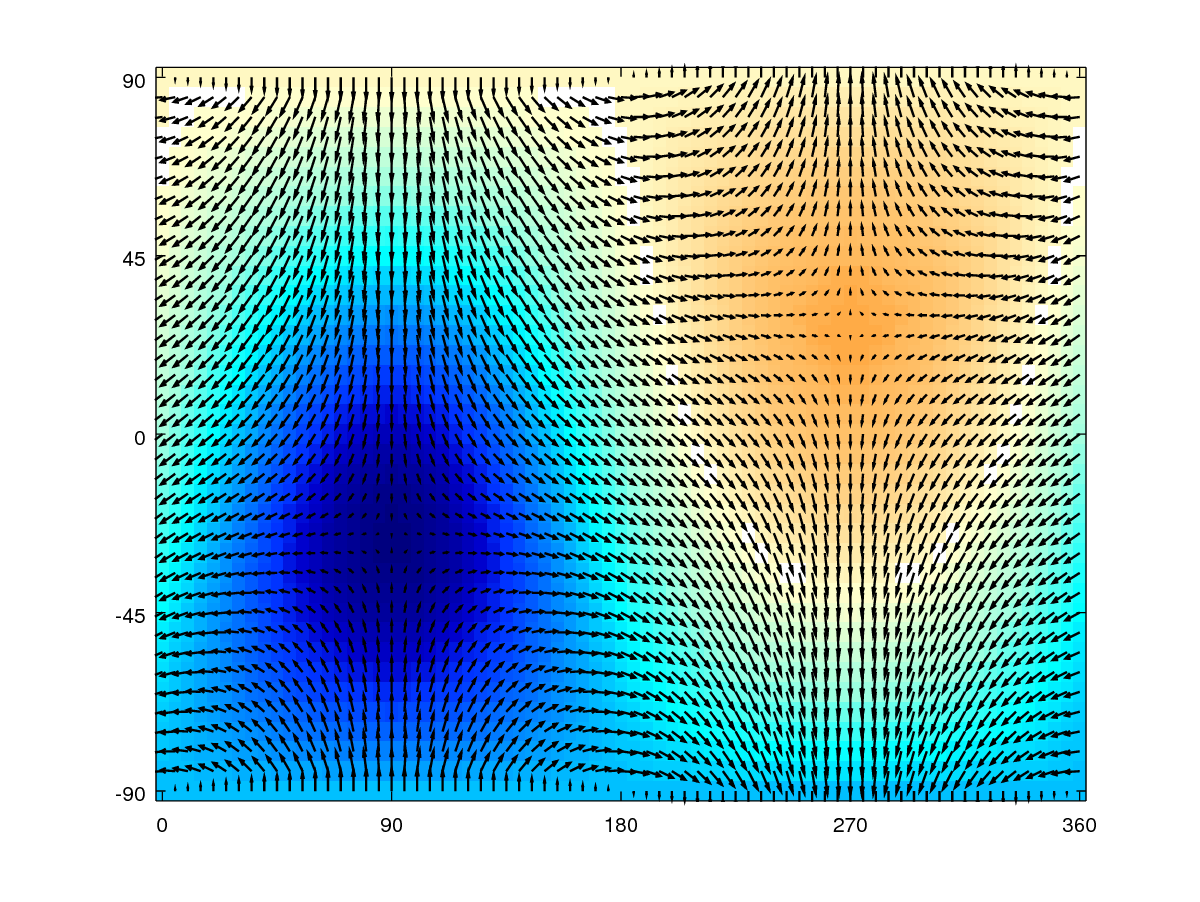
\includegraphics[width=0.5\textwidth]{figures_Rep2/lincomb2.png}  
  \caption{Linear combination of the vector spherical harmonics $2E_{00}-1.5E_{10}+3E_{11}$, with known coefficients to calculate the spherical harmonic functions.}
\label{E_knowncoeff}
\end{figure}

\subsection{Linear Combinations with $E_{lm}$, $F_{lm}$, and $C_{lm}$:}

If the vector field is represented as a linear combination of $E_{lm}$, $F_{lm}$, and $C_{lm}$, then we will need to evaluate each of the spherical harmonics separately then sum them.  We can calculate $F_{lm}$ by running:

\verb|L = 2;|\\
\verb|theta = 0:0.01:pi;|\\
\verb|phi = 0:0.01:2*pi;|\\
\verb|[F,theta,phi] = flm(L,theta,phi);|

Say we have a linear combination $E_{10}+F_{11}$ and we want to just look at the radial component.  We can evaluate the spherical harmonics at the $(l,m)$ combination.  Run:

\verb|lincomb = E{1}(3,:)+F{1}(4,:);|\\
\verb|lincombr = reshape(lincomb,length(theta),length(phi));|

Plot this on the Mallweide projection:

\verb|plotplm(lincombr,phi+pi,pi/2-theta,1)|\\
\verb|kelicol(1)|

Compare your plot to figure 6.
\begin{figure}[H]
  \centering
  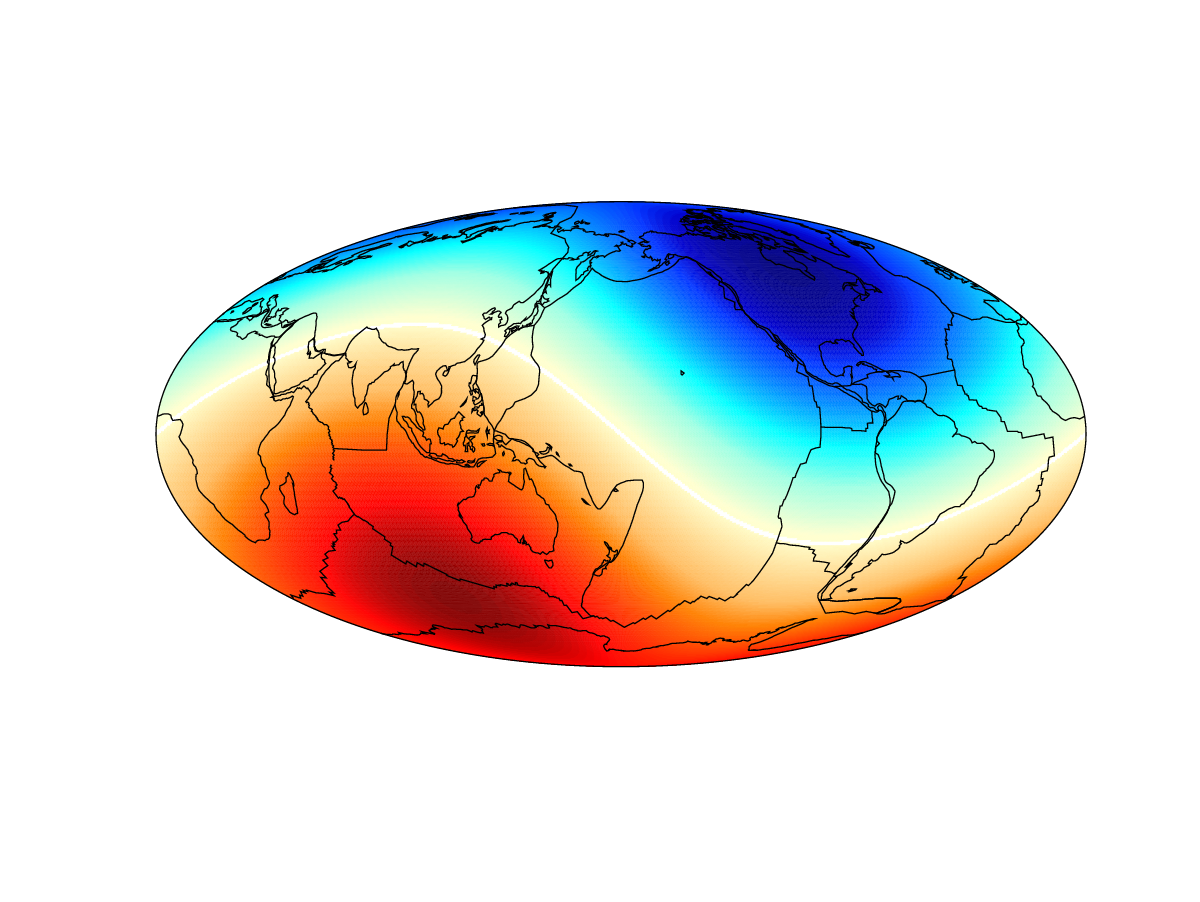
\includegraphics[width=0.5\textwidth]{figures_Rep2/lincombEF1.png}  
  \caption{Radial linear combination of the vector spherical harmonics $E_{10}+F_{11}$.}
\label{EFcomb}
\end{figure}

We can also create the linear combinations with the colatitudinal and longitudinal components.  Lower the resolution and recalculate $E_{lm}$, $F_{lm}$, and the linear combinations for each component:

\verb|theta = 0:0.1:pi;|\\
\verb|phi = 0:0.1:2*pi;|\\
\verb|lincomb_theta = E{2}(3,:)+F{2}(4,:);|\\
\verb|lincombr_theta = reshape(lincomb_theta,length(theta),length(phi));|\\
\verb|lincomb_phi = E{3}(3,:)+F{3}(4,:);|\\
\verb|lincombr_phi = reshape(lincomb_phi,length(theta),length(phi));|

Now let's plot these components using the \verb|quiver| function, as before:

\verb|plotplm(lincombr,phi,pi/2-theta,4)|\\
\verb|kelicol(1)|\\
\verb|hold on|\\
\verb|quiver(phi*180/pi-180,90-theta*180/pi,lincombr_phi,lincombr_theta,'k','LineWidth',1)|\\
\verb|hold off|

Compare your plot to 7 of the linear combination.
\begin{figure}[H]
  \centering
  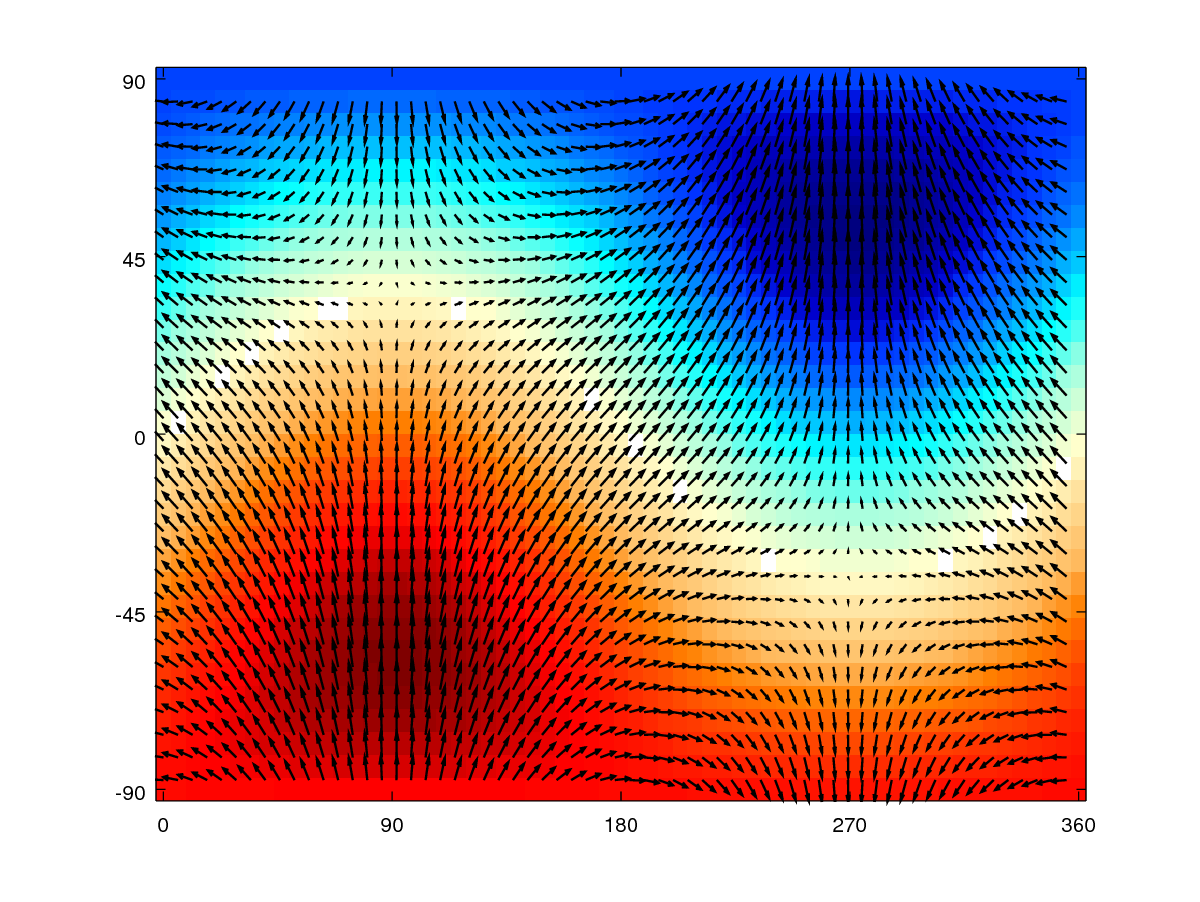
\includegraphics[width=0.5\textwidth]{figures_Rep2/lincombEF_quiver.png}  
  \caption{Linear combination of the vector spherical harmonics $E_{10}+F_{11}$.}
\label{EFcomb_quiver}
\end{figure}

We can also create linear combinations with $C_{lm}$.  Since $C_{lm}$ is calculated by taking one $(l,m)$ combination, let's choose and run:

\verb|theta = 0:0.1:pi;|\\
\verb|phi = 0:0.1:2*pi;|\\
\verb|l = 1;|\\
\verb|m = -1;|\\
\verb|[B,C,theta,phi] = blmclm(l,m,theta,phi);|

We will need to create a linear combination first for the radial component, which $C_{lm}$ does not contain, so run:

\verb|lincomb_rad = E{2}(2,:)+F{2}(2,:);|\\
\verb|lincombr_rad = reshape(lincomb_rad,length(theta),length(phi));|

Let's create a linear combination with all three $E_{lm}$, $F_{lm}$, and $C_{lm}$. 
We must reshape the components first since $E_{lm}$ and $F_{lm}$ contain pixel map information in a vector, while $C_{lm}$ contains the information in a matrix.

\verb|E1m1_theta=reshape(E{2}(2,:),length(theta),length(phi));|\\
\verb|E1m1_phi=reshape(E{3}(2,:),length(theta),length(phi));|\\
\verb|F1m1_theta=reshape(F{2}(2,:),length(theta),length(phi));|\\
\verb|F1m1_phi=reshape(F{3}(2,:),length(theta),length(phi));|

Now we can create the linear combinations:

\verb|lincomb_theta = E1m1_theta+F1m1_theta+C{1};|\\
\verb|lincomb_phi = E1m1_phi+F1m1_phi+C{2};|

Now we can plot this:

\verb|plotplm(lincombr_rad,phi,pi/2-theta,4)|\\
\verb|kelicol(1)|\\
\verb|hold on|\\
\verb|quiver(phi*180/pi,90-theta*180/pi,lincomb_phi,lincomb_theta,'k','LineWidth',1)|\\
\verb|hold off|

Figure 8 shows the plot of this linear combination.
\begin{figure}[H]
  \centering
  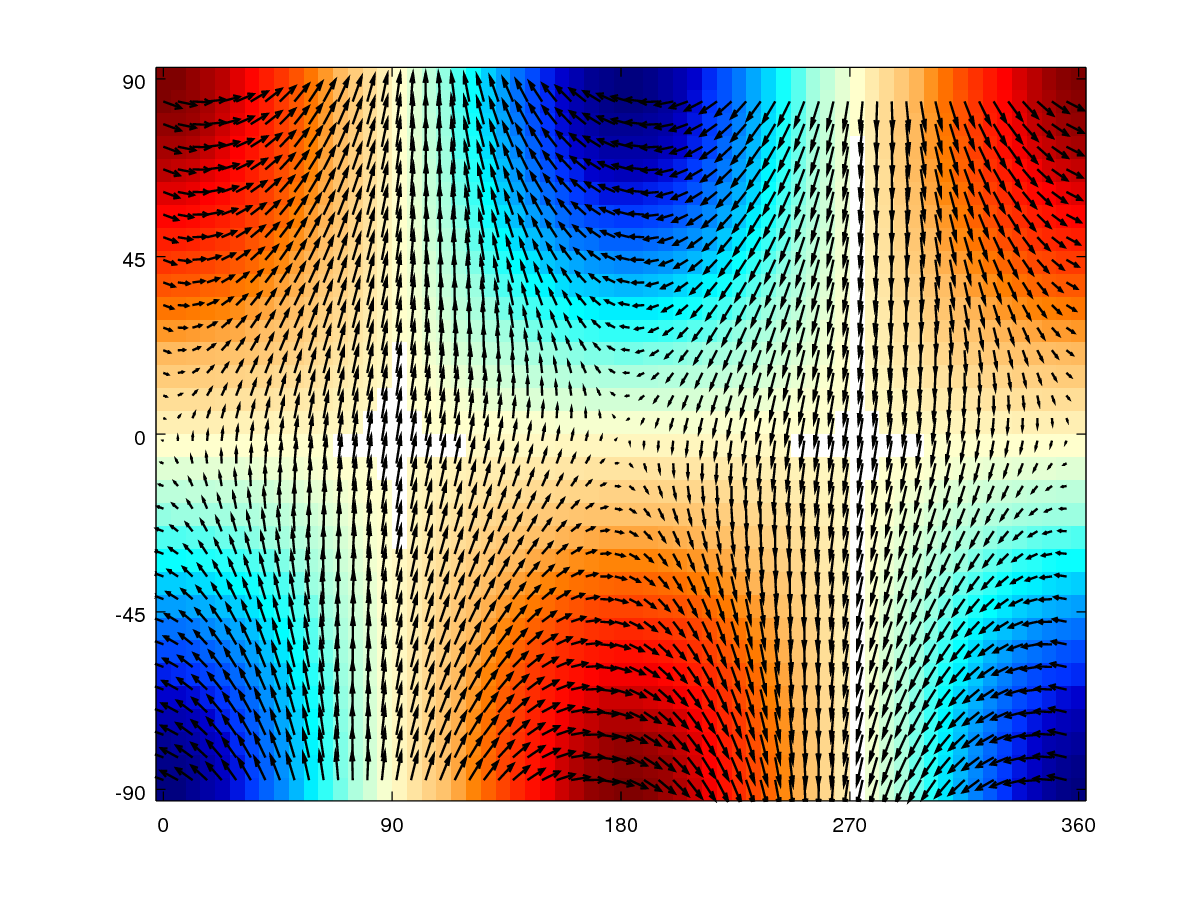
\includegraphics[width=0.5\textwidth]{figures_Rep2/lincombEFC_quiver.png}  
  \caption{Linear combination of the vector spherical harmonics $E_{1-1}+F_{1-1}+C_{1-1}$ with l=1 and m=-1.}
\label{EFCcomb_quiver}
\end{figure}




\HERE

\TAG
\end{document}